\documentclass{article}

\usepackage{fancyhdr}
\usepackage{extramarks}
\usepackage{amsmath}
\usepackage{amsthm}
\usepackage{amsfonts}
\usepackage{tikz}
\usepackage[plain]{algorithm}
\usepackage{algpseudocode}
\usepackage{graphicx}
\usepackage{gensymb}
\usepackage{hyperref}

\DeclareRobustCommand{\bbone}{\text{\usefont{U}{bbold}{m}{n}1}}

\DeclareMathOperator{\EX}{\mathbb{E}}% expected value

\graphicspath{{./images/}}

\usetikzlibrary{automata,positioning}

%
% Basic Document Settings
%

\topmargin=-0.45in
\evensidemargin=0in
\oddsidemargin=0in
\textwidth=6.5in
\textheight=9.0in
\headsep=0.25in

\linespread{1.1}

\pagestyle{fancy}
\lhead{\hmwkAuthorName}
\chead{\hmwkClassShort\ \hmwkTitle}
\rhead{\firstxmark}
\lfoot{\lastxmark}
\cfoot{\thepage}

\renewcommand\headrulewidth{0.4pt}
\renewcommand\footrulewidth{0.4pt}

\setlength\parindent{0pt}

%
% Create Problem Sections
%

\newcommand{\enterProblemHeader}[1]{
    \nobreak\extramarks{}{Problem {#1} continued on next page\ldots}\nobreak{}
    \nobreak\extramarks{{#1} (continued)}{{#1} continued on next page\ldots}\nobreak{}
}

\newcommand{\exitProblemHeader}[1]{
    \nobreak\extramarks{{#1} (continued)}{{#1} continued on next page\ldots}\nobreak{}
    % \stepcounter{#1}
    \nobreak\extramarks{{#1}}{}\nobreak{}
}

\setcounter{secnumdepth}{0}
\newcounter{partCounter}

\newcommand{\problemNumber}{0.0}

\newenvironment{homeworkProblem}[1][-1]{
    \renewcommand{\problemNumber}{{#1}}
    \section{\problemNumber}
    \setcounter{partCounter}{1}
    \enterProblemHeader{\problemNumber}
}{
    \exitProblemHeader{\problemNumber}
}

%
% Homework Details
%   - Title
%   - Class
%   - Author
%

\newcommand{\hmwkTitle}{DRL Assignment}
\newcommand{\hmwkClassShort}{RBE 595}
\newcommand{\hmwkClass}{RBE 595 --- Reinforcement Learning}
\newcommand{\hmwkAuthorName}{\textbf{Arjan Gupta}}

%
% Title Page
%

\title{
    \vspace{2in}
    \textmd{\textbf{\hmwkClass}}\\
    % \textmd{\textbf{\hmwkTitle}}\\
    \textmd{\textbf{Deep Reinforcement Learning Assignment}}\\
    \vspace{3in}
}

\author{\hmwkAuthorName}
\date{}

\renewcommand{\part}[1]{\textbf{\large Part \Alph{partCounter}}\stepcounter{partCounter}\\}

%
% Various Helper Commands
%

% Useful for algorithms
\newcommand{\alg}[1]{\textsc{\bfseries \footnotesize #1}}

% For derivatives
\newcommand{\deriv}[2]{\frac{\mathrm{d}}{\mathrm{d}#2} \left(#1\right)}

% For compact derivatives
\newcommand{\derivcomp}[2]{\frac{\mathrm{d}#1}{\mathrm{d}#2}}

% For partial derivatives
\newcommand{\pderiv}[2]{\frac{\partial}{\partial #2} \left(#1\right)}

% For compact partial derivatives
\newcommand{\pderivcomp}[2]{\frac{\partial #1}{\partial #2}}

% Integral dx
\newcommand{\dx}{\mathrm{d}x}

% Alias for the Solution section header
\newcommand{\solution}{\textbf{\large Solution}}

% Probability commands: Expectation, Variance, Covariance, Bias
\newcommand{\E}{\mathrm{E}}
\newcommand{\Var}{\mathrm{Var}}
\newcommand{\Cov}{\mathrm{Cov}}
\newcommand{\Bias}{\mathrm{Bias}}

\begin{document}

\maketitle

\nobreak\extramarks{Problem 1}{}\nobreak{}

\pagebreak

\begin{homeworkProblem}[Problem 1]
    What are the two sources of error in Deep RL with function approximation?

    \subsection{Answer}

    The two sources of error in Deep RL with function approximation are as follows:

    \begin{itemize}
        \item \textbf{Bootstrapping error} --- This is the error that arises due to the use of
        bootstrapping. Bootstrapping is the process of using the value of a successor state to
        update the value of a state. This is done in TD methods. The error is the difference
        between the target value and the current estimate value.
        \item \textbf{Approximation error} --- This is the error defined as the difference
        between the true value function and the approximate value function. This error arises
        due to the use of function approximation itself.
    \end{itemize}

\end{homeworkProblem}

\nobreak\extramarks{Problem 2}{}\nobreak{}

\pagebreak

\begin{homeworkProblem}[Problem 2]
    We mentioned that the target value for TD is $[R_{t+1} + \gamma V(s_{t+1})]$. What is the target value for
    Monte-carlo, Q-learning, SARSA and Expected-SARSA?

    \subsection{Answer}

    The Target is shown as part of the following equation:
    \begin{align*}
        NewEstimate \leftarrow OldEstimate + StepSize \left[ Target - OldEstimate \right]
    \end{align*}

    \begin{itemize}
        \item \textbf{Monte-Carlo} (MC) does not use bootstrapping. Its target value is the
        actual return value, $G_t$.
        \item \textbf{Q-Learning} --- As given in the algorithm, the target value is
        $R_{t+1} + \gamma \max_{a} Q(S_{t+1}, a)$.
        \item \textbf{SARSA} --- As shown in the algorithm, the target value is
        $R_{t+1} + \gamma Q(S_{t+1}, A_{t+1})$.
        \item \textbf{Expected-SARSA} --- As described in the book, the target value is
        $R_{t+1} + \gamma \mathbb{E}_{\pi} \left[ Q(S_{t+1}, A_{t+1}) \mid S_{t+1} \right]$.
    \end{itemize}

\end{homeworkProblem}

\nobreak\extramarks{Problem 2}{}\nobreak{}

\pagebreak

\nobreak\extramarks{Problem 3}{}\nobreak{}

\begin{homeworkProblem}[Problem 3]
    What are the similarities of TD and MC\@?

    \subsection{Answer}

    The similarities between TD and MC are as follows:

    \begin{itemize}
        \item Both TD and MC are model-free, i.e. they do not require a model of the environment.
        \item Both TD and MC are \textit{sample updates}, i.e., they involve looking ahead at a sample
        successor state (or state-action pair), using the value of that state to compute a backed-up value, and then updating
        the value of the original state (or state-action pair) accordingly.
    \end{itemize}
\end{homeworkProblem}

\pagebreak

\nobreak\extramarks{Problem 4}{}\nobreak{}

\begin{homeworkProblem}[Problem 4]
    Assume that we have two states $x$ and $y$ with the current value of $V(x) = 10$, $V(y) = 1$. We
    run an episode of $\{x, 3, y, 0, y, 5, T\}$. What's the new estimate of $V(x)$, $V(y)$ using TD (assume
    step size $\alpha = 0.1$ and discount rate $\gamma = 0.9$).

    \subsection{Answer}

    The new estimate of $V(x)$ is as follows:

    \begin{align*}
        V(x) &= V(x) + \alpha \left[ R_{t+1} + \gamma V(S_{t+1}) - V(x) \right]\\
             &= 10 + 0.1 \left[ 3 + 0.9 \cdot 1 - 10 \right]\\
             &= 10 + 0.1 \left[ 3.9 - 10 \right]\\
             &= 10 + 0.1 \left[ -6.1 \right]\\
             &= 10 - 0.61\\
             &= 9.39
    \end{align*}

    However, $V(y)$ gets updated twice in this episode. The first update is as follows:

    \begin{align*}
        V(y) &= V(y) + \alpha \left[ R_{t+1} + \gamma V(S_{t+1}) - V(y) \right]\\
             &= 1 + 0.1 \left[ 0 + 0.9 \cdot 1 - 1 \right]\\
                &= 1 + 0.1 \left[ 0.9 - 1 \right]\\
                &= 1 + 0.1 \left[ -0.1 \right]\\
                &= 1 - 0.01\\
                &= 0.99
    \end{align*}

    The second update is as follows:

    \begin{align*}
        V(y) &= V(y) + \alpha \left[ R_{t+1} + \gamma V(S_{t+1}) - V(y) \right]\\
             &= 0.99 + 0.1 \left[ 5 + 0.9 \cdot 0 - 0.99 \right]\\
                &= 0.99 + 0.1 \left[ 5 - 0.99 \right]\\
                &= 0.99 + 0.1 \left[ 4.01 \right]\\
                &= 0.99 + 0.401\\
                &= 1.391
    \end{align*}

    Therefore, the new estimate of $V(x)$ is $9.39$ and the new estimate of $V(y)$ is $1.391$.

\end{homeworkProblem}

\pagebreak

\nobreak\extramarks{Problem 5}{}\nobreak{}

\begin{homeworkProblem}[Problem 5]
    Can we consider TD an online (real-time) method and MC an offline method? Why?

    \subsection{Answer}
    
    Yes, we can consider TD an online (real-time) method and MC an offline method. This is because
    TD learns during the episode, whereas MC learns after the episode has ended. Specifically, TD updates the
    value of a state based on the value of the next state (during the episode), whereas MC updates
    the value of a state based on successive returns (after the episode has ended).
\end{homeworkProblem}

\pagebreak

\nobreak\extramarks{Problem 6}{}\nobreak{}

\begin{homeworkProblem}[Problem 6]

    Does Q-learning learn the outcome of exploratory actions? (Refer to the Cliff walking example).

    \subsection{Answer}

    Yes, Q-learning learns the outcome of exploratory actions. This is because Q-learning is an
    off-policy TD control algorithm. In the context of the Cliff walking example, this means that
    Q-learning learns the optimal action-value function, $q_*$, which is closest to the cliff. 
    The behavior policy takes exploratory actions, and the target policy is greedy. This
    causes makes it so that initially, the agent falls off the cliff a lot, but eventually, the agent
    learns to avoid the cliff and converges to the optimal action-value function, $q_*$. This is why the
    graph of the sum of rewards per episode for Q-learning is initially very low, but eventually
    converges to a high value. The graph is shown below:

    \begin{center}
        % 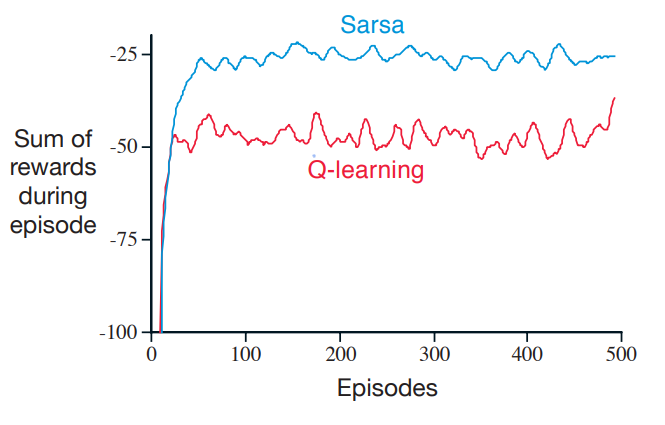
\includegraphics[scale=0.5]{q_learning_cliff_walking.png}
    \end{center}

\end{homeworkProblem}

\pagebreak

\nobreak\extramarks{Problem 7}{}\nobreak{}

\begin{homeworkProblem}[Problem 7]

    What is the advantage of Double Q-learning over Q-learning?

    \subsection{Answer}

    The advantage of Double Q-learning over Q-learning is that Double Q-learning is less prone to
    bias than Q-learning. Specifically, Q-learning is biased toward the maximum value action, which
    is also known as maximization bias. This is because Q-learning uses the maximum value action
    to update the value of a state.\\

    In contrast, Double Q-learning is not biased toward the maximum value action. This is because
    Double Q-learning uses two action-value functions, $Q_1$ and $Q_2$, to update the value of a state.
    With probability $0.5$, Double Q-learning uses either $Q_1$ or $Q_2$ to update the value of a state.
    Now, for example, the action is picked as per $Q_1$, then that action is probably not the maximum
    value action as per $Q_2$. This way, for a given state, we have two estimates of the value of the
    maximum value action. This reduces the bias of Double Q-learning and is hence the advantage over
    Q-learning.


\end{homeworkProblem}

\end{document}